\textbf{\large\color{orange}Zadanie 5.} Mapą na powierzchni $M$ nazywamy podział powierzchni na komórki homeomorficzne z dyskami, których przekroje są zawarte w ich brzegach. Z takim podziałem
mamy związany graf dualny, którego wierzchołki, to komórki, a krawędź istnieje
pomiędzy wierzchołkami, gdy odpowiadające im komórki mają niepusty przekrój.
Kolorowaniem mapy nazywać będziemy funkcję ze zbioru komórek w pewien skończony zbiór kolorów, która przyjmuje różne wartości na krojących się niepusto
komórkach.
\begin{enumerate}[label=(\alph*)]
  \item Jak mogą wyglądać mapy na powierzchniach? Czy da się uprościć je tak, by
graf dualny był $1$-szkieletem triangulacji? Rozważyć mapę o sześciu krajach
na butelce Kleina.
\item Twierdzenie o $k$ barwach dla powierzchni $M$ mówi, że każdą mapę na powierzchni $M$ można pokolorować co najwyżej $k$ kolorami. Udowodnić twierdzenie o $5$ barwach dla sfery $S^2$, o $6$ barwach dla $RP^2$ o $7$ barwach dla torusa
$T^2$ i o $6$ barwach dla butelki Kleina.
\end{enumerate}

\dotfill 

\begin{enumerate}[label=\textbf{(\alph*)}]
  \item W mapie pozwalamy, aby w jednym punkcie spotykały się co najwyżej $3$ kraje. Jeśli istnieje punkt, w którym spotykają się $4$ kraje, wtedy ten punkt zamieniamy na krawędź:
    \begin{center}\begin{tikzpicture}
      \fill [pattern={Dots[radius=1pt, distance=6pt, xshift=0.5mm]}, pattern color=pink!80!blue] (-1.5, -1.5) rectangle ++(1.5, 1.5);
      \fill [pattern={Stars[points=4, radius=2pt, distance=6pt, xshift=-1mm]}, pattern color=orange!40!red] (0, -1.5) rectangle ++(1.5, 1.5);
      \fill [pattern={Hatch[angle=45, distance=4pt]}, pattern color=green!70!orange] (-1.5, -3) rectangle ++(1.5, 1.5);
      \fill [pattern={Lines[distance=4pt, angle=45]}] (0, -3) rectangle ++(1.5, 1.5);

      \fill[opacity=0.6, white] (-1.5,-3) rectangle ++(3, 3);


      \draw[thick] (0, 0)--(0, -3);
      \draw[thick] (-1.5, -1.5)--(1.5, -1.5);


      \fill [pattern={Dots[radius=1pt, distance=6pt, xshift=0.2mm]}, pattern color=pink!80!blue] (4.7, 0)--(4.7, -1.3)--(4.3, -1.7)--(3, -1.7)--(3, 0)--cycle;
      \fill [pattern={Stars[points=4, radius=2pt, distance=6pt, xshift=0mm]}, pattern color=orange!40!red] (4.7, 0)--(4.7, -1.3)--(6, -1.3)--(6, 0)--cycle;
      \fill [pattern={Hatch[angle=45, distance=4pt]}, pattern color=green!70!orange] (3, -1.7)--(4.3, -1.7)--(4.3, -3)--(3, -3)--cycle;
      \fill [pattern={Lines[distance=4pt, angle=45]}] (4.3, -3)--(4.3, -1.7)--(4.7, -1.3)--(6, -1.3)--(6, -3)--cycle;

      \fill[opacity=0.6, white] (3, 0) rectangle (6, -3);

      \draw[thick] (4.7, 0)--(4.7, -1.3)--(6, -1.3);
      \draw[thick] (3, -1.7)--(4.3, -1.7)--(4.3, -3);
      \draw[thick] (4.3, -1.7)--(4.7, -1.3);

      \draw[style={decorate, decoration=snake}, thick] (1.7, -1.5)--(2.8, -1.5);
      \draw[thick, ->] (2.86, -1.5)--(2.88, -1.5);

      \coordinate (A1) at (-0.75, -0.75);
      \coordinate (A2) at (0.75, -.75);
      \coordinate (A3) at (0.75, -2.25);
      \coordinate (A4) at (-0.75, -2.25);

    \fill (A1) circle (2pt);
  \fill (A2) circle (2pt);
\fill(A3) circle (2pt);
\fill(A4) circle (2pt);
      
      \draw[very thick, blue](A1)--(A2)--(A3)--(A4)--(A1);

      \coordinate(B1) at (4, -0.75);
      \coordinate(B2) at (5.5, -0.75);
      \coordinate(B3) at (5, -2.25);
      \coordinate(B4) at (3.5, -2.25);

      \draw[very thick, blue] (B1)--(B2)--(B3)--(B4)--(B1);
      \draw[very thick, blue] (B1)--(B3);

    \fill (B1) circle (2pt);
  \fill (B2) circle (2pt);
\fill(B3) circle (2pt);
\fill(B4) circle (2pt);
    \end{tikzpicture}\end{center}
    W ten sposób z grafu $C_4$ dostajemy graf mający trójkąty jako ściany.

    W przypadku, gdy widzimy na mapie Andorę, to ignorujemy jedną granicę między Francją i Hiszpanią przy rysowaniu grafu dualnego: \def\r{1.5}
    \begin{center}\begin{tikzpicture}
      \fill[pattern={Lines[distance=4pt, angle=80]}, pattern color=orange] (-5, 3) rectangle (0, -3);
      \fill[pattern={Hatch[angle=45, distance=4pt]}, pattern color=green] (0, -3) rectangle (5, 3);
      \fill[white] (0,0) circle (\r);
      \fill[pattern={Dots[radius=1pt, distance=6pt, angle=45]}, pattern color=pink] (0,0) circle (\r);

      \draw[thick] (0,0) circle (\r);

      \draw[thick] (0, 3)--(0, \r);
      \draw[thick] (0, -\r)--(0, -3);

      \coordinate (A) at (-3.5, 2);
      \coordinate (B) at (3.5, 2);
      \coordinate (C) at (0, 0);

      \draw[very thick, blue] (A)--(C)--(B)--(A);

      \fill (A) circle (2pt);
      \fill (B) circle (2pt);
      \fill (C) circle (2pt);
    \end{tikzpicture}\end{center}
    Unikamy w ten sposób krawędzi wielokrotnych. % i dostajemy miejsce na dwuwymiarowy sympleks ($\triangle$).


    Niestety, nie każdy graf pochodzący od takich map na powierzchni da się rozszerzyć do triangulacji. Rozważmy na przykład mapę, do której graf dualny to $K_6$ na butelce Kleina:
    \begin{center}\begin{tikzpicture}[
line cap=round,
marr/.style={
  decoration={
    markings,
    mark=at position 0.5 with {#1}
    },
  postaction={decorate}
}
] 
    \begin{scope}[shift={(-5, 0)}]

    \fill[green] (-2, 2) rectangle (0,0);
    \fill[yellow] (-2, 0) rectangle (0, -2); 
    \fill[blue] (2, 2)--(2, 1)--(0,0)--(0, 2)--cycle;
    \fill[purple] (0, 0)--(2, 1)--(2, -2)--(-0.5, -2)--(0,0);
    \fill[pink] (2, 1)--(2, -1)--(1, -1)--(0,0)--(1, 1)--cycle;

    \fill[orange] (0,0) circle (0.7);

    \foreach \i in {1,...,5}
    \fill (\i*360/5:1.5) coordinate (n\i) circle(2 pt);
      %\ifnum \i>1 foreach \j in {\i,...,1}{(n\i) edge (n\j)} \fi;
    \fill (0,0) circle (2pt);
    \foreach \i in {1,...,5} \draw (0, 0)--(n\i);

    \draw[black, thick] (n1)--(0.1, 2);
    \draw[black, thick] (-0.1, -2)--(n4);

    \draw[black, thick] (n1)--(0.7, 2);
    \draw[black, thick] (-0.7, -2)--(n3);

    %\draw[blue, thick] (n1)--(2, 1.15);
    %\draw[blue, thick] (-2, 1.15)--(n2);
    
    \draw[black, thick] (n2)--(-2, 0.45);
    \draw[black, thick] (2, 0.45)--(n5);

    \draw[black, thick] (n5)--(2, -0.45);
    \draw[black, thick] (-2, -0.45)--(n3);

    \draw[black, thick] (n4)--(0.7, -2);
    \draw[black, thick] (-0.7, 2)--(n2);

    \draw (n1)--(n2)--(n3)--(n4)--(n5)--(n1);
  \fill[opacity=0.7, white] (-2, 2) rectangle (2, -2);

\path
  coordinate (n1) at (-2,-2)
  coordinate (n2) at (-2,2)
  coordinate (n3) at (2,-2)
  coordinate (n4) at (2,2);
\foreach \from/\to in {n1/n3,n4/n2}
    \draw[marr=\Singlearrow] (\from) -- (\to);
\foreach \from/\to in {n1/n2,n3/n4}
    \draw[marr=\Doublearrow] (\from) -- (\to);

\end{scope}



\path
  coordinate (n1) at (-2,-2)
  coordinate (n2) at (-2,2)
  coordinate (n3) at (2,-2)
  coordinate (n4) at (2,2);
\foreach \from/\to in {n1/n3,n4/n2}
    \draw[marr=\Singlearrow] (\from) -- (\to);
\foreach \from/\to in {n1/n2,n3/n4}
    \draw[marr=\Doublearrow] (\from) -- (\to);

    \foreach \i in {1,...,5}
    \fill (\i*360/5:1.5) coordinate (n\i) circle(2 pt);
      %\ifnum \i>1 foreach \j in {\i,...,1}{(n\i) edge (n\j)} \fi;
    \fill (0,0) circle (2pt);
    \foreach \i in {1,...,5} \draw (0, 0)--(n\i);

    \fill[pattern={Dots[angle=45, radius=1pt, distance=6pt]}, pattern color=orange] (n4)--(n5)--(2, -0.45)--(2, -2)--(0.7, -2)--cycle;
    \fill[pattern={Dots[angle=45, radius=1pt, distance=6pt]}, pattern color=orange] (n3)--(-0.7, -2)--(-2, -2)--(-2, -0.45)--cycle;
    \fill[pattern={Dots[angle=45, radius=1pt, distance=6pt]}, pattern color=orange] (n1)--(n5)--(2, 0.45)--(2, 2)--(0.7, 2)--cycle;
    \fill[pattern={Dots[angle=45, radius=1pt, distance=6pt]}, pattern color=orange] (n2)--(-2, 0.45)--(-2, 2)--(-0.7, 2)--(n2)--cycle;

    \draw[blue, thick] (n1)--(0.1, 2);
    \draw[blue, thick] (-0.1, -2)--(n4);

    \draw[blue, thick] (n1)--(0.7, 2);
    \draw[blue, thick] (-0.7, -2)--(n3);

    %\draw[blue, thick] (n1)--(2, 1.15);
    %\draw[blue, thick] (-2, 1.15)--(n2);
    
    \draw[blue, thick] (n2)--(-2, 0.45);
    \draw[blue, thick] (2, 0.45)--(n5);

    \draw[blue, thick] (n5)--(2, -0.45);
    \draw[blue, thick] (-2, -0.45)--(n3);

    \draw[blue, thick] (n4)--(0.7, -2);
    \draw[blue, thick] (-0.7, 2)--(n2);

    \draw (n1)--(n2)--(n3)--(n4)--(n5)--(n1);

    %\node at (n1) {$1$};

    \end{tikzpicture}\end{center}
    Obszar zacieniowany kółeczkami po prawej stronie rysunku zawiera $5$ wierzchołków zamiast $3$ zwyczajowo obecnych w $\triangle$. Nie możemy tego pięciokąta przekroić by otrzymać trójkąty, bo $K_6$ jest już grafem pełnym i takie działanie dałoby wielokrotną krawędź.


  \item 

    \textbf{Torus} $\mathbf{T^2}$\dotfill

    Zacznijmy od tego, że $7$ kolorów na torusie jest koniecznych. Wynika to z faktu, że triangulacja torusa o minimalnej ilości wierzchołków to $K_7$.

    Po pierwsze, minimalna ilość wierzchołków w triangulacji na torusie to $7$. Ponieważ torus jest rozmaitością $2$ wymiarową, to
    $$2E=3T$$
    $$\frac{2}{3}E=T$$
    z formuły Gaussa-Bonnet wiemy, że
    $$0=V-E+F=V-E+\frac{2}{3}E=V-\frac{1}{3}E.\quad (\star)$$
    Górne szacowanie na ilość wierzchołków to
    $$E\leq \binom{V}{2}=\frac{V(V-1)}{2},$$
    co po podstawieniu do $(\star)$ daje
    $$0=V-\frac{1}{3}E\geq V-\frac{V(V-1)}{6}=\frac{7V-V^2}{6}=\frac{V(7-V)}{6}$$
    co implikuje, że $V\geq 7$.

    \begin{center}\begin{tikzpicture}[
line cap=round,
marr/.style={
  decoration={
    markings,
    mark=at position 0.5 with {#1}
    },
  postaction={decorate}
}
] 
\path
  coordinate (n1) at (-2,-2)
  coordinate (n2) at (-2,2)
  coordinate (n3) at (2,-2)
  coordinate (n4) at (2,2);
\foreach \from/\to in {n1/n3,n2/n4}
    \draw[marr=\Singlearrow] (\from) -- (\to);
\foreach \from/\to in {n1/n2,n3/n4}
    \draw[marr=\Doublearrow] (\from) -- (\to);


\coordinate (A1) at (-2, -2);
\coordinate (A2) at (-2, 2);
\coordinate (A3) at  (2, -2);
\coordinate (A4) at (2,2);

\coordinate (B1) at (-2, {2-4/3});
\coordinate (B2) at (2, {2-4/3});

\coordinate (C1) at (-2, {-2+4/3});
\coordinate (C2) at (2, {-2+4/3});

\coordinate (D1) at ({2-4/3}, 2);
\coordinate (D2) at ({2-4/3}, -2);

\coordinate (E1) at ({-2+4/3}, 2);
\coordinate (E2) at ({-2+4/3}, -2);

\coordinate (F) at ({2-4/3}, {2-4/3});
\coordinate (G) at ({-2+4/3}, {-2+4/3});

\draw (A1)--(G)--(F)--(A4);
\draw (D1)--(F)--(B2);
\draw (C1)--(G)--(E2);

\draw (C2)--(D2)--(G)--(B2);
\draw (D2)--(B2);

\draw (F)--(C1)--(E1)--(B1);
\draw (F)--(E1);

    \fill[green] (-2, -2) circle (3pt);
    \fill[green] (-2, 2) circle (3pt);
    \fill[green] (2, -2) circle (3pt);
    \fill[green] (2,2) circle (3pt);

    \fill[orange] (-2, {2-4/3}) circle (3pt);
    \fill[blue] (-2, {-2+4/3}) circle (3pt);

    \fill[orange] (2, {2-4/3}) circle (3pt);
    \fill[blue] (2, {-2+4/3}) circle (3pt);

    \fill[pink] ({2-4/3}, 2) circle (3pt);
    \fill ({-2+4/3}, 2) circle (3pt);

    \fill[pink] ({2-4/3}, -2) circle (3pt);
    \fill ({-2+4/3}, -2) circle (3pt);

    \fill[yellow] ({2-4/3}, {2-4/3}) circle (3pt);
    \fill[purple] ({-2+4/3}, {-2+4/3}) circle (3pt);

    \end{tikzpicture}\end{center}

    Pokażemy teraz, przy pomocy indukcji po ilości wierzchołków, że dla każdego grafu $G$ na torusie wystarczy $7$ kolorów, by go pomalować. 

    Przypadek bazowy, to znaczy $|G|\leq 7$, jest dość oczywisty. Załóżmy teraz, że każdy graf o co najwyżej $n$ wierzchołkach potrafimy pokolorować $7$ kolorami. Niech $G$ będzie grafem na torusie, który ma $(n+1)$ wierzchołków. Rozważamy przypadki:
    \begin{enumerate}[label=\arabic*.]
      \item Istnieje wierzchołek $v\in G$ taki, że $\deg(v)\leq6$.

        Możemy wtedy wierzchołek $v$ wyjąć, tzn. rozważyć graf $G'=G\setminus v$ w którym ze zbioru wierzchołków usunięty został $v$, a ze zbioru krawędzi usunięto wszystkie krawędzie $e$ takie, że $e\cap v\neq \emptyset$.

        Na mocy założenia indukcyjnego graf $G'$ możemy pokolorować $7$ kolorami. Sąsiedzi wierzchołka $v$, jako że było ich $6$ sztuk, korzystają z maksymalnie $6$ kolorów. Możemy więc wybrać kolor, który nie jest przez nich użyty i pomalować nim $v$.

      \item Jeśli wszystkie wierzchołki mają stopień co najmniej $7$, to wtedy mamy 
        $$E=\frac{1}{2}\sum_{v\in V}\deg(v)\geq \frac{7V}{2}\implies \frac{2}{7}E\geq V$$ 
        krawędzi. 

        Graf $G$ niekoniecznie jest triangulacją, ale na pewno nie zawiera przecinających się krawędzi. Możemy więc nieco zmodyfikować to, co wiemy o zależności między liczbą krawędzi a liczbą ścian. Jesteśmy na rozmaitości dwuwymiarowej, więc jedna krawędź trafia do dwóch ścian. Każda ściana z kolei ma co najmniej $3$ krawędzie. Dostajemy więc zależność
        $$2E\geq 3T\implies \frac{2}{3}E\geq T.$$

        Charakterystyka Eulera torusa wynosi $0$, więc możemy użyć formuły Gaussa-Bonneta
        \begin{align*}
          0&=V-E+T\leq V-E+\frac{2}{3}E=\\ 
                 &=V-\frac{1}{3}E\leq\frac{2}{7}E-\frac{1}{3}E=\\ 
                 &=\frac{6-7}{21}E=-\frac{E}{21}
        \end{align*}
        z tego wynika, że
        $$0\geq {E}$$
        co daje sprzeczność z $E>0$. W takim razie w grafie narysowanym na torusie zawsze znajdziemy wierzchołek stopnia $\leq 6$.
    \end{enumerate}

    \textbf{Płaszczyzna rzutowa $\boldsymbol{\R}\mathbf{ P^2}$} \dotfill

    Zaczniemy znowu od pokazania, że istnieje na $\R P^2$ graf, który potrzebuje $6$ kolorów do bycia pomalowanym.

    Triangulacja $\R P^2$ o najmniejszej liczbie wierzchołków to $K_6$. Wnioskujemy to z formuły Gaussa-Bonnet uzupełnionej o fakt, że $\R P^2$ jest rozmaitością wymiaru $2$
    $$1=V-E+T=V-\frac{1}{3}E$$
    dokładamy jeszcze górne ograniczenie na liczbę krawędzi, czyli $E\leq\binom{V}{2}$, by dostać
    $$1=V-\frac{1}{3}E\geq V-\frac{V(V-1)}{6}=\frac{V(7-V)}{6}$$
    $$0\leq \frac{6+V(V-7)}{6}$$
    $V=6$ jest najmniejszym dodatnim rozwiązaniem tej nierówności.

    Dla $V=6$ wymagamy $E=15$, czyli $6$-wierzchołkowa triangulacja $\R P^2$ jest grafem $K_6$:
    %\def{\v1}{pink}\def{\v2}{green}\def{\v3}{blue}\def{\v4}{pink}\def{\v5}{green}\def{\v6}{blue}
    \begin{center}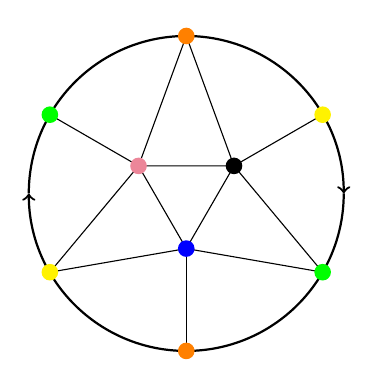
\begin{tikzpicture}
      \draw[->, thick] (-2, 0) arc (180:0:2);
      \draw[->, thick] (2, 0) arc (0:-180:2);

      \foreach \c [count=\i] in {orange, green, yellow, orange, green, yellow} {
        \fill[\c] (\i*360/6+360/12:2) circle (2pt); 
        \coordinate (n\i) at (\i*360/6+360/12:2);
      }

      \foreach \i in {1,...,3} {
        \fill (\i*360/3 + 30:0.7) circle (2pt);
        \coordinate (m\i) at (\i * 120 + 30:0.7);
      }

      \draw (m1)--(m2)--(m3)--(m1);
      \draw (m1)--(n1)--(m3);
      \draw (m1)--(n3)--(m2);
      \draw (m2)--(n5)--(m3);
      \draw (m1)--(n2);
      \draw (m2)--(n4);
      \draw (m3)--(n6);

      \foreach \c [count=\i] in {orange, green, yellow, orange, green, yellow} 
        \fill[\c] (\i*360/6+360/12:2) circle (3pt); 

      \foreach \c [count=\i] in {pink!70!purple, blue, black} 
      \fill[\c] (\i*360/3 + 30:0.7) circle (3pt);
    \end{tikzpicture}\end{center}

    Załóżmy teraz, że wszystkie grafy o co najwyżej $n$ wierzchołkach narysowane na $\R P^2$ potrafimy pomalować używając $6$ kolorów. Niech $G$ będzie grafem o $(n+1)$ wierzchołkach. 
    \begin{enumerate}[label=\arabic*.]
      \item Jeśli istnieje wierzchołek $v\in G$ taki, że $\deg(v)\leq 5$, to podobnie jak w przypadku torusa, możemy ten wierzchołek wyjąć, pokolorować graf $G'=G\setminus v$ i znajdziemy dla $v$ kolor niewykorzystywany przez jego sąsiadów.
      \item W tym przypadku zakładamy, że wszystkie wierzchołki $v\in G$ mają stopień $\deg(v)\geq 6$. Tak jak i wcześniej, mamy
        $$2E\geq 3T$$
        $$2E\geq 6V.$$
        Płaszczyzna rzutowa ma charakterystykę Eulera $1$, w takim razie
        $$1=V-E+T$$
        $$3=3V-3E+3T\leq E-3E+2E=0$$
        co jest sprzecznością. W takim razie w grafie narysowanym na $\R P^2$ zawsze znajdziemy wierzchołek $\deg(v)\leq 5$ i wykonamy kroki z pierwszego punktu.
    \end{enumerate}
%    Dalej mamy rozmaitość $2$ wymiarową, więc $2E=3T$. Z formuły Gaussa-Bonneta dostajemy
%    $$1=\sum_{v\in V}(1-\frac{e_v}{v})=V-\frac{1}{3}E.$$
%
%    Mapy mające $\leq 6$ krajów nie są problemem, więc weźmy mapę o $(n+1)$ krajach. Znowu, robimy z niej graf dualny, który musi być planarny. Możemy więc odrysować krawędzie tak, by otrzymać triangulację. Wiemy, że w grafie zachodzi
%    $$E=\frac{1}{2}\sum_{v\in V}deg(v).$$
%    Co, jeśli nasz $(n+1)$ wierzchołkowy graf ma tylko wierzchołki stopnia $6$ lub więcej? Wtedy
%    $$E\geq \frac{1}{2}\sum_{v\in V}6=\frac{1}{2}\cdot 6V=3V.$$
%    Wracając z tym szacowaniem do formuły G-B dostalibyśmy
%    $$1=V-\frac{1}{3}E\leq V-\frac{1}{3}\cdot 3V=V-V=0$$
%    co jest zdecydowaną sprzecznością. Stąd musi istnieć wierzchołek stopnia $5$ lub mniej i możemy go wyciąć, pomalować resztę i wybrać mu kolor różny od koloru użytego przez co najwyżej $5$ jego sąsiadów.
%
    \textbf{Sfera $\mathbf{S^2}$} \dotfill

    W przypadku sfery próżno szukać grafu, którego nie pokolorujemy $4$ kolorami - prawdziwe jest twierdzenie o $4$ barwach.

    Oczywiście grafy, które mają nie więcej niż $5$ wierzchołków pokolorujemy bez problemu. Załóżmy więc, że każdy graf o co najwyżej $n$ wierzchołkach możemy pokolorować i niech $G$ będzie $(n+1)$-wierzchołkowym grafem.

    \begin{enumerate}[label=\arabic*]
      \item Jeśli znajdziemy wierzchołek stopnia $\leq 4$ lub mniej to robimy to co w przypadku torusa i płaszczyzny rzutowej.
      \item Jeśli istnieje wierzchołek $v\in G$ stopnia $5$.
        \begin{enumerate}
          \item 
        Jeśli $v$ ma $2$ sąsiadów, którzy nie są ze sobą połączeni, wtedy po wyjęciu $v$ możemy złączyć ich w jeden wierzchołek:
        \begin{center}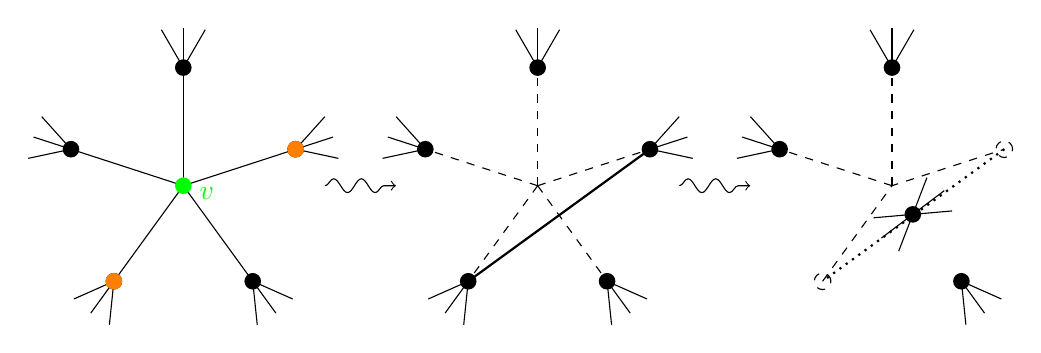
\begin{tikzpicture}
        \foreach \i in {1,...,5} {
          \fill (\i*72+18:1.5) circle (3pt);
          \draw (0,0)--(\i*72+18:1.5);
        \draw (\i*72+18:1.5)--(\i*72+18:2);
        \draw (\i*72+18:1.5)--(\i*72+10:2);
        \draw (\i*72+18:1.5)--(\i*72+26:2);
        }

        \fill[orange] (18:1.5) circle (3.01pt);
        \fill[orange] (18-2*72:1.5) circle (3.01pt);


          \fill[green] (0,0) circle (3pt);
          \node[green] at (0.3, -0.1) {$v$};

          \draw[style={decorate, decoration=snake}, ->] (1.8, 0)--(2.7, 0);

          \begin{scope}[shift={(4.5, 0)}]
            \foreach \i in {1,...,5} {
              \fill (\i*72+18:1.5) circle (3pt);
              \draw[dashed] (0,0)--(\i*72+18:1.5);
        \draw (\i*72+18:1.5)--(\i*72+18:2);
        \draw (\i*72+18:1.5)--(\i*72+10:2);
        \draw (\i*72+18:1.5)--(\i*72+26:2);
            }
            \draw[thick] (18:1.5)--(18-2*72:1.5);
          \end{scope}

          \draw[style={decorate, decoration=snake}, ->] (6.3, 0)--(7.2, 0);
          
          \begin{scope}[shift={(9, 0)}]
            \foreach \i in {1,...,2} {
              \fill (\i*72+18:1.5) circle (3pt);
              \draw[dashed] (0,0)--(\i*72+18:1.5);
        \draw (\i*72+18:1.5)--(\i*72+18:2);
        \draw (\i*72+18:1.5)--(\i*72+10:2);
        \draw (\i*72+18:1.5)--(\i*72+26:2);
            }
          \fill (18-72:1.5) circle (3pt);
          \draw [dashed] (18-2*72:1.5)--(0,0)--(18:1.5);
          \draw[dashed] (18:1.5) circle (3pt);
          \draw[dashed] (18-2*72:1.5) circle (3pt);
            \draw[thick, dotted] (18:1.5)--(18-2*72:1.5);
          %\fill(18-72:0.45) circle (3pt);

          \begin{scope}[shift={(18-72:0.45)}]
          \fill (0,0) circle (3pt);
          \draw (0,0)--(72-35:0.5);
          \draw (0,0)--(104-35:0.5);
          \draw (0,0)--(40-35:0.5);

          \draw (0,0)--(72-35+180:0.5);
          \draw (0,0)--(104-35+180:0.5);
          \draw (0,0)--(40-35+180:0.5);
          \end{scope}

        \draw (18-72:1.5)--(-72+18:2);
        \draw (-72+18:1.5)--(-72+10:2);
        \draw (-72+18:1.5)--(-72+26:2);
          \end{scope}
        \end{tikzpicture}\end{center}
        Po takiej operacji nadal mamy graf narysowany na $S^2$, bo tylko wciągnęliśmy w pustkę pozostawioną przez $v$ krawędzie.

        Taki graf jak na skrajnie prawym rysunku ma $(n-2)$ wierzchołki, więc możemy go pomalować $5$ kolorami. Dwóch sąsiadów $v$ zlepiliśmy w jedno i pokolorowaliśmy tym samym kolorem, więc po ich rozczepieniu nadal mogą mieć ten sam kolor. $v$ miało $5$ sąsiadów, którzy używają nie więcej niż $4$ kolorów - możemy pozostały kolor użyć na $v$.

      \item Jeśli wszyscy sąsiedzi $v$ są ze sobą połączeni, to wtedy $G$ ma podgraf będący $K_5$. 

        Sfera to tak naprawdę punkt z doczepionym dyskiem $D^2$, czyli jeśli wytniemy wokół $v$ dysk zawierający wszystkich jego sąsiadów, to możemy go rozprostować i patrzeć na ten podgraf narysowany na płaszczyźnie. Jednak twierdzenie Kuratowskiego (o grafach) mówi, że na płaszczyźnie możemy narysować graf $\iff$ nie zawiera podgrafu izomorficznego z $K_5$ ani z $K_{3,3}$. Stąd ten przypadek jest niemożliwy.
    \end{enumerate}
  \item Jeśli każdy wierzchołek $v\in G$ ma stopień $>5$, to dostaniemy sprzeczność z formułą Gaussa-Bonnet. Ilość krawędzi szacujemy z jeden strony przez stopień wierzchołków:
    $$2E=\sum_{v\in V}\deg(v)\geq\sum_{v\in V}6=6V$$
    $$E\geq 3V$$
    a z drugiej przez fakt, że każda krawędź leży w dwóch ścianach, a każda ściana ma co najmniej $3$ krawędzie:
    $$2E\geq 3T.$$
    Wstawiając to do formuły Gaussa-Bonnet z pamięcią, że $\chi(S^2)=2$, dostajemy
    $$2=V-E+T$$
    $$6=3V-3E+3T\leq E-3E+2E=0$$
    czyli sprzeczność.
    \end{enumerate}

    \textbf{Butelka Kleina} \dotfill

  Rozważmy graf $G$ na butelce Kleina. Jeśli $|G|\leq 6$, to bez problemy pokolorujemy go $6$ kolorami (fakt, że potrzebujemy co najmniej $6$ kolorów wynika z rysunku w ptk (a) zadania). 

  Niech więc $G$ będzie grafem na butelce Kleina. 
  \begin{enumerate}[label=\arabic*]
    \item Jeśli istnieje wierzchołek $v\in G$ taki, że $\deg(v)\leq 5$, to możemy ten wierzchołek wyjąć, pokolorować $6$ kolorami graf $G\setminus \{v\}$, wierzchołek $v$ pomalować kolorem, który nie pojawia się wśród jego $\leq 5$ sąsiadów i włożymy go z powrotem do $G$ nie psując kolorowania.

    \item Zadanie komplikuje się natomiast, jeśli $G$ jest $6$-regularny. Wybierzmy wierzchołek $v\in G$. Ma on $6$ sąsiadów, czyli jest wierzchołkiem $6$ trójkątów w triangulacji którą stał się $G$:
  \begin{center}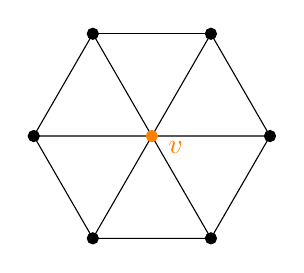
\begin{tikzpicture}
    \draw (-1.5, 0)--({-1.5*cos(60)}, {1.5*sin(60)})--(0,0)--({1.5*cos(60)}, {1.5*sin(60)})--(1.5, 0)--(0,0)--({1.5*cos(60)}, {-1.5*sin(60)})--({-1.5*cos(60)}, {-1.5*sin(60)})--(0,0)--cycle;
    \draw ({-1.5*cos(60)}, {1.5*sin(60)})--({1.5*cos(60)}, {1.5*sin(60)});
    \draw (1.5, 0)--({1.5*cos(60)}, {-1.5*sin(60)});
    \draw ({-1.5*cos(60)}, {-1.5*sin(60)})--(-1.5,0);

      %({1.5*cos(60)}, {-1.5*sin(60)})--({-1.5*cos(60)}, {-1.5*sin(60)})--cycle;
\filldraw (1.5, 0) circle (2pt);
\filldraw(-1.5, 0) circle (2pt);
\filldraw({-1.5*cos(60)}, {1.5*sin(60)}) circle (2pt);
\filldraw({1.5*cos(60)}, {1.5*sin(60)}) circle (2pt);
\filldraw({-1.5*cos(60)}, {-1.5*sin(60)}) circle (2pt);
\filldraw({1.5*cos(60)}, {-1.5*sin(60)}) circle (2pt);

\filldraw[orange](0,0) circle(2pt);
\node at (0.3, -0.15) {$\color{orange}v$};
  \end{tikzpicture}\end{center}
  Jeżeli istnieje para sąsiadów, która nie jest ze sobą połączona, to możemy pomalować je na jeden kolor. Wtedy sąsiedzi $v$ wykorzystują tylko $5$ kolorów i ostatni, szósty, pozostaje wolny do kolorowania $v$. 

  Jeśli natomiast wszyscy sąsiedzi $v$ są ze sobą połączeni, to oznacza, że mamy $K_7$ zanurzone w $G$, które z kolei jest narysowane na butelce Kleina. Wiemy, że $K_7$ nie można narysować na butelce Kleina, więc dochodzimy do sprzeczności w tym punkcie.
\item Jeśli w $G$ istnieje wierzchołek stopnia $7$ a pozostałe wierzchołki mają stopień $\deg(v)\geq6$, to możemy użyć Gaussa-Bonnet, by dostać sprzeczność.

  Tak jak wcześniej, szacujemy ilość krawędzi na dwa sposoby:
  $$2E= \sum_{v\in V}\deg(v)\geq 6(V-1)+7=6V+1$$
  $$2E\geq 3T$$
  wstawiamy to do formuły Gaussa-Bonneta i dostajemy
  $$0=V-E+T$$
  $$0=6V-6E+6T\leq (2E-1)-6E+4E=6E-6E-1=-1$$
  $$0\leq -1$$
  co jest sprzecznością.
\end{enumerate}
\end{enumerate}
